\documentclass[fleqn,11pt]{article}
\usepackage[letterpaper,margin=0.75in]{geometry}
\usepackage{amsmath}
\usepackage{booktabs}
\usepackage{graphicx}
\usepackage{listings}
\usepackage{caption}
\usepackage{tikz}
\usepackage{circuitikz}
\setlength{\parindent}{1.4em}

\begin{document}


\title{Coursework2}
\author{Yuli Zhi fh19804}
\date{}
\maketitle
\section*{Question 1}
\begin{center}
    \centering
    \captionof{table}{Fano Factor}
    \begin{tabular}{|l|l|l|}
    \hline
    Window Width & no refractory period & 5ms refractory period \\ \hline
    10ms                               & 1.004830592459605                                                                                  &  0.7495329181494661                                        \\ \hline
    50ms                               & 1.0129321364452424                                                                                  & 0.6911521352313167                                         \\ \hline
    100ms                              & 1.0072938061041292                                                                                  & 0.690688612099644                                         \\ \hline
    \end{tabular}
\end{center}
\par Coefficient of variation with no refractory period:1.008257526709267
\par Coefficient of variation with 50ms refractory period:0.824144815535471


\section*{Question 2}
\par The calculation uses data of rho.dat
\begin{center}
    \centering
    \captionof{table}{Fano Factor and CoV}
    \begin{tabular}{|l|l|l|}
    \hline
    Window Width/Cov & Results  \\ \hline
    10ms                               & 1.117680142627936   \\ \hline
    50ms                               & 2.9297562848640877  \\ \hline
    100ms                              & 4.102959520344769   \\ \hline
    Coefficient of variation           & 2.0085154091296     \\ \hline
    \end{tabular}
\end{center}

\section*{Question 3}
    \begin{center} 
        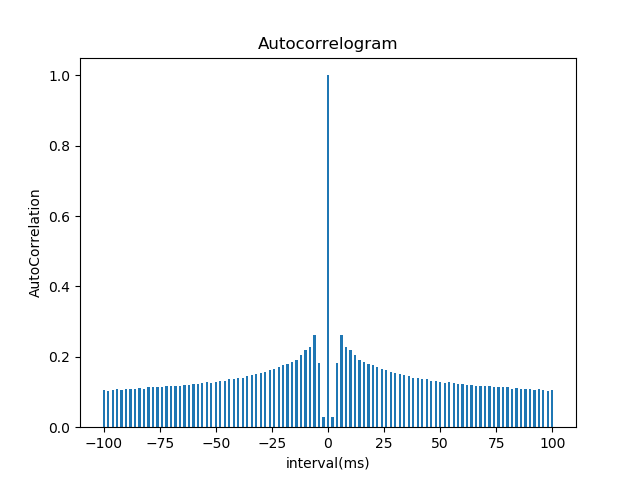
\includegraphics[width=10cm]{graphs/Autocorrelogram.png}
        \captionof{figure}{Autocorrelogram at [-100,100]ms}
    \end{center}
\section*{Question 4}
\begin{center} 
    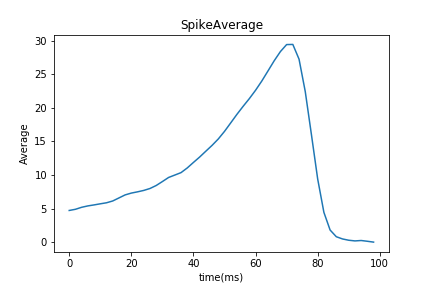
\includegraphics[width=10cm]{graphs/SpikeAverage.png}
    \captionof{figure}{SpikeAverage over 100ms windows}
\end{center}
\section*{Question COMSM2127}
\par Multiple-Spike-Triggered average.
     The plot shows the average stimulus before two spikes with 
     a interval of 2ms, 10ms, 20ms, 50ms, and both the case 
     where the spikes are not necessarily adjacent and the case where they are.
    \begin{center} 
        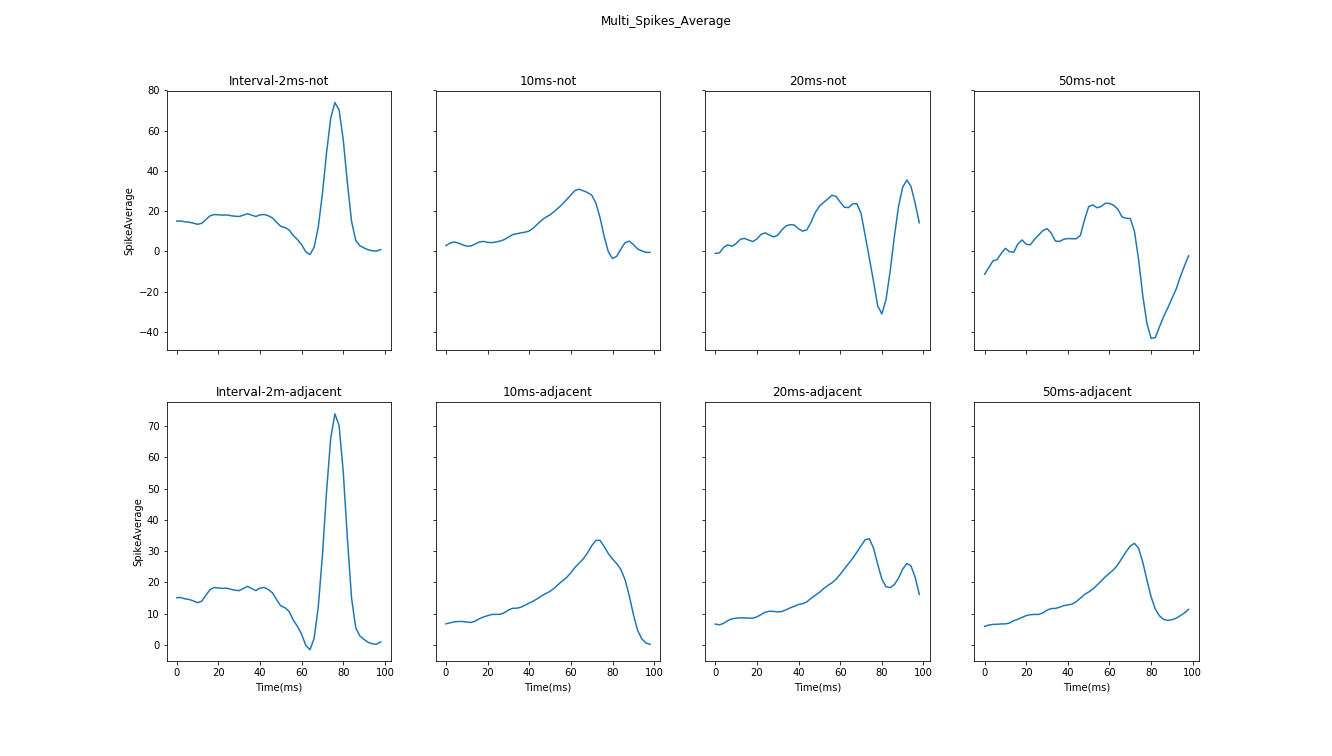
\includegraphics[width=15cm]{graphs/MultiAverage.png}
        \captionof{figure}{MultiAverage: Interval: 2ms,10ms,20ms,50ms}
    \end{center}
\end{document}



